\documentclass[12pt,a4paper]{article}

% Paquetes esenciales para artículos de Ciberseguridad
\usepackage{cite}
\usepackage{amsmath,amssymb,amsfonts}
\usepackage{algorithm}
\usepackage{algpseudocode}
\usepackage{graphicx}
\usepackage{textcomp}
\usepackage{xcolor}
\usepackage{booktabs}
\usepackage{array}
\usepackage{multirow}
\usepackage{siunitx}
\usepackage{listings}
\usepackage{float}

\usepackage{tikz}
\usetikzlibrary{shapes,arrows,positioning,fit,backgrounds,calc}
\usepackage{pgfplots}

\pgfplotsset{compat=1.16}

\usepackage{hyperref}
\usepackage{tabularx}
\usepackage{enumitem}
\usepackage{mdframed}
\usepackage[left=2.5cm,right=2.5cm,top=2.5cm,bottom=2.5cm]{geometry}
\usepackage{authblk} % Para gestionar autores y afiliaciones de manera sencilla

\usepackage[spanish]{babel} % idioma en español


% Definición de colores para ciberseguridad
\definecolor{alertred}{RGB}{235,54,42}
\definecolor{warningyellow}{RGB}{250,190,40}
\definecolor{securegreen}{RGB}{46,204,113}
\definecolor{infoblue}{RGB}{52,152,219}
\definecolor{vulnerablepurple}{RGB}{155,89,182}
\definecolor{codegray}{RGB}{240,240,240}
\definecolor{commentgreen}{RGB}{63,127,95}
\definecolor{codeblue}{RGB}{0,0,255}
\definecolor{codered}{RGB}{176,0,0}
\definecolor{cryptogreen}{RGB}{0,128,0}
\definecolor{encryptionbg}{RGB}{245,245,245}

% Configuración para listings con soporte mejorado para Python
\lstdefinestyle{pythoncode}{
    language=Python,
    basicstyle=\ttfamily\small,
    keywordstyle=\color{codeblue}\bfseries,
    stringstyle=\color{codered},
    commentstyle=\color{commentgreen}\itshape,
    showstringspaces=false,
    numbers=left,
    numberstyle=\tiny\color{gray},
    numbersep=5pt,
    frame=single,
    backgroundcolor=\color{codegray},
    breaklines=true,
    breakatwhitespace=true,
    tabsize=4,
    captionpos=b
}

% Definición para mostrar algoritmos criptográficos o pseudocódigo
\lstdefinestyle{cryptoalgo}{
    basicstyle=\ttfamily\small,
    keywordstyle=\color{cryptogreen}\bfseries,
    stringstyle=\color{codered},
    commentstyle=\color{commentgreen}\itshape,
    showstringspaces=false,
    numbers=left,
    numberstyle=\tiny\color{gray},
    numbersep=5pt,
    frame=single,
    backgroundcolor=\color{encryptionbg},
    breaklines=true,
    breakatwhitespace=true,
    tabsize=4,
    captionpos=b,
    emphstyle=\color{blue},
    emph={permutación, expansión, sustitución, rotación, desplazamiento, cifrado, descifrado, bloque, ronda, clave}
}

\lstset{style=pythoncode}

% Estilos para bloques de alerta de seguridad
\newmdenv[
  linecolor=alertred,
  backgroundcolor=alertred!10,
  frametitle={Alerta de Seguridad},
  frametitlebackgroundcolor=alertred!40,
  frametitlefont=\bfseries\color{white},
  roundcorner=4pt
]{securityalert}

\newmdenv[
  linecolor=warningyellow,
  backgroundcolor=warningyellow!10,
  frametitle={Advertencia},
  frametitlebackgroundcolor=warningyellow!40,
  frametitlefont=\bfseries\color{black},
  roundcorner=4pt
]{securitywarning}

\newmdenv[
  linecolor=securegreen,
  backgroundcolor=securegreen!10,
  frametitle={Buena Práctica},
  frametitlebackgroundcolor=securegreen!40,
  frametitlefont=\bfseries\color{white},
  roundcorner=4pt
]{securitygoodpractice}

% Definición para métodos criptográficos
\newmdenv[
  linecolor=infoblue,
  backgroundcolor=infoblue!5,
  frametitle={Método Criptográfico},
  frametitlebackgroundcolor=infoblue!40,
  frametitlefont=\bfseries\color{white},
  roundcorner=4pt
]{cryptomethod}

% Definición para análisis criptográfico
\newmdenv[
  linecolor=vulnerablepurple,
  backgroundcolor=vulnerablepurple!5,
  frametitle={Análisis Criptográfico},
  frametitlebackgroundcolor=vulnerablepurple!40,
  frametitlefont=\bfseries\color{white},
  roundcorner=4pt
]{cryptoanalysis}

% Definición de BibTeX
\def\BibTeX{{\rm B\kern-.05em{\sc i\kern-.025em b}\kern-.08em
    T\kern-.1667em\lower.7ex\hbox{E}\kern-.125emX}}

\begin{document}

\title{\LARGE \textbf{Laboratorio: Programación Segura\\Suite de Cifrado Criptográfico}}

\author{\textbf{Profesor Gustavo Adolfo Echeverri\\}}
\author[1]{Juan Carlos Charfuelan Caipe}
\author[2]{Fabian Alberto Guancha Vera}
\author[3]{Over Haider Castrillón Valencia}

\affil[1]{Departamento de Ingeniería en Sistemas y Computación, Universidad de Caldas}
\affil[Manizales, Colombia}
\date{\today}
\maketitle

\section*{Introducción}
Este laboratorio presenta la implementación de una suite completa de cifrado utilizando las bibliotecas criptográficas de Python. Se abordan conceptos fundamentales de la criptografía moderna incluyendo funciones hash, firmas digitales, cifrado simétrico y asimétrico, y criptografía de curvas elípticas. Cada implementación se acompaña de explicaciones teóricas, código funcional y análisis de seguridad.

\tableofcontents
\newpage

\section{Configuración del Entorno}

\subsection{Requisitos del Sistema}
Para ejecutar las implementaciones presentadas en este laboratorio, se
requiere:

\begin{itemize}
	\item Python 3.8 o superior
	\item Bibliotecas criptográficas: \texttt{cryptography}, \texttt{pycryptodome}
	\item Sistema operativo: Windows, Linux o macOS
\end{itemize}

\subsection{Instalación de Dependencias}

\begin{lstlisting}[language=bash, caption=Instalación de bibliotecas requeridas]
pip install cryptography pycryptodome
\end{lstlisting}

\begin{securitygoodpractice}
	Se recomienda utilizar un entorno virtual de Python para aislar las dependencias del proyecto y evitar conflictos con otros paquetes instalados en el sistema.
\end{securitygoodpractice}

\newpage

\section{Resumen Digital (Message Digest)}

\subsection{Fundamentos Teóricos}

Un resumen digital o función hash criptográfica es una función matemática que
convierte datos de entrada de longitud arbitraria en una salida de longitud
fija. Las propiedades fundamentales incluyen:

\begin{itemize}
	\item \textbf{Determinista}: La misma entrada siempre produce la misma salida
	\item \textbf{Eficiencia computacional}: Rápida de calcular
	\item \textbf{Resistencia a preimagen}: Computacionalmente infactible encontrar una entrada que produzca un hash específico
	\item \textbf{Resistencia a colisiones}: Extremadamente difícil encontrar dos entradas diferentes que produzcan el mismo hash
	\item \textbf{Efecto avalancha}: Pequeños cambios en la entrada producen cambios significativos en la salida
\end{itemize}

\subsection{Implementación}

\begin{cryptomethod}
	La implementación utiliza múltiples algoritmos de hash para demostrar las diferencias en longitud de salida y aplicaciones prácticas.
\end{cryptomethod}

\begin{lstlisting}[caption=Implementación de funciones hash criptográficas]
import hashlib
from typing import Dict, Union

class MessageDigest:
    """
    Clase para generar resúmenes digitales usando diferentes algoritmos hash.
    """
    
    def __init__(self):
        self.supported_algorithms = ['md5', 'sha1', 'sha256', 'sha384', 'sha512', 'sha3_256', 'sha3_512']
        
    def generate_hash(self, message: Union[str, bytes], algorithm: str = 'sha256') -> str:
        """
        Genera un hash del mensaje usando el algoritmo especificado.
        
        Args:
            message: Mensaje a hashear (string o bytes)
            algorithm: Algoritmo a utilizar (default: sha256)
            
        Returns:
            Hash hexadecimal del mensaje
        """
        if algorithm not in self.supported_algorithms:
            raise ValueError(f"Algoritmo {algorithm} no soportado")
            
        # Convertir string a bytes si es necesario
        if isinstance(message, str):
            message = message.encode('utf-8')
            
        # Crear objeto hash según el algoritmo
        if algorithm == 'md5':
            hash_obj = hashlib.md5()
        elif algorithm == 'sha1':
            hash_obj = hashlib.sha1()
        elif algorithm == 'sha256':
            hash_obj = hashlib.sha256()
        elif algorithm == 'sha384':
            hash_obj = hashlib.sha384()
        elif algorithm == 'sha512':
            hash_obj = hashlib.sha512()
        elif algorithm == 'sha3_256':
            hash_obj = hashlib.sha3_256()
        elif algorithm == 'sha3_512':
            hash_obj = hashlib.sha3_512()
            
        # Actualizar con el mensaje y retornar el hash
        hash_obj.update(message)
        return hash_obj.hexdigest()
    
    def compare_algorithms(self, message: str) -> Dict[str, str]:
        """
        Compara los resultados de diferentes algoritmos hash.
        
        Args:
            message: Mensaje a hashear
            
        Returns:
            Diccionario con los resultados de cada algoritmo
        """
        results = {}
        for algo in self.supported_algorithms:
            results[algo] = {
                'hash': self.generate_hash(message, algo),
                'length': len(self.generate_hash(message, algo))
            }
        return results
    
    def verify_integrity(self, message: str, expected_hash: str, algorithm: str = 'sha256') -> bool:
        """
        Verifica la integridad de un mensaje comparando su hash.
        
        Args:
            message: Mensaje a verificar
            expected_hash: Hash esperado
            algorithm: Algoritmo utilizado
            
        Returns:
            True si el hash coincide, False en caso contrario
        """
        calculated_hash = self.generate_hash(message, algorithm)
        return calculated_hash == expected_hash

# Ejemplo de uso
if __name__ == "__main__":
    md = MessageDigest()
    
    # Ejemplo básico
    mensaje = "Este es un mensaje de prueba para el laboratorio"
    hash_sha256 = md.generate_hash(mensaje)
    print(f"SHA-256 del mensaje: {hash_sha256}")
    
    # Comparación de algoritmos
    print("\nComparación de algoritmos:")
    comparacion = md.compare_algorithms(mensaje)
    for algo, data in comparacion.items():
        print(f"{algo}: {data['hash'][:32]}... (longitud: {data['length']})")
    
    # Verificación de integridad
    print("\nVerificación de integridad:")
    es_integro = md.verify_integrity(mensaje, hash_sha256)
    print(f"Mensaje íntegro: {es_integro}")
    
    # Demostración del efecto avalancha
    mensaje_modificado = "Este es un mensaje de prueba para el Laboratorio"
    hash_modificado = md.generate_hash(mensaje_modificado)
    print(f"\nMensaje original: {hash_sha256}")
    print(f"Mensaje modificado (cambio de 'l' a 'L'): {hash_modificado}")
    print(f"Hashes iguales: {hash_sha256 == hash_modificado}")
\end{lstlisting}

\begin{securitywarning}
	MD5 y SHA-1 ya no se consideran seguros para aplicaciones criptográficas debido a vulnerabilidades conocidas. Se recomienda usar SHA-256 o superior para aplicaciones que requieren seguridad.
\end{securitywarning}

\subsection{Análisis de Seguridad}

\begin{cryptoanalysis}
	Los algoritmos hash modernos como SHA-256 y SHA-3 proporcionan seguridad robusta contra ataques conocidos. La longitud de salida determina la resistencia a ataques de fuerza bruta:
	\begin{itemize}
		\item SHA-256: $2^{256}$ posibles salidas
		\item SHA-512: $2^{512}$ posibles salidas
	\end{itemize}
\end{cryptoanalysis}

\newpage

\section{Firma Digital}

\subsection{Fundamentos Teóricos}

La firma digital es un esquema matemático que demuestra la autenticidad de un
mensaje digital. Proporciona:

\begin{itemize}
	\item \textbf{Autenticación}: Verifica la identidad del firmante
	\item \textbf{Integridad}: Garantiza que el mensaje no ha sido alterado
	\item \textbf{No repudio}: El firmante no puede negar haber firmado el mensaje
\end{itemize}

El proceso involucra:
\begin{enumerate}
	\item Generación de un par de claves (pública y privada)
	\item Creación de un hash del mensaje
	\item Cifrado del hash con la clave privada (firma)
	\item Verificación descifrando con la clave pública
\end{enumerate}

\subsection{Implementación RSA}

\begin{lstlisting}[caption=Implementación de firma digital con RSA]
from cryptography.hazmat.primitives import hashes, serialization
from cryptography.hazmat.primitives.asymmetric import rsa, padding
from cryptography.hazmat.backends import default_backend
from cryptography.exceptions import InvalidSignature
import base64

class DigitalSignature:
    """
    Clase para implementar firma digital usando RSA.
    """
    
    def __init__(self, key_size: int = 2048):
        """
        Inicializa el sistema de firma digital.
        
        Args:
            key_size: Tamaño de la clave RSA (default: 2048 bits)
        """
        self.key_size = key_size
        self.private_key = None
        self.public_key = None
        
    def generate_keys(self):
        """
        Genera un par de claves RSA.
        """
        self.private_key = rsa.generate_private_key(
            public_exponent=65537,
            key_size=self.key_size,
            backend=default_backend()
        )
        self.public_key = self.private_key.public_key()
        
    def sign_message(self, message: bytes) -> bytes:
        """
        Firma un mensaje usando la clave privada.
        
        Args:
            message: Mensaje a firmar
            
        Returns:
            Firma digital del mensaje
        """
        if not self.private_key:
            raise ValueError("No se ha generado la clave privada")
            
        signature = self.private_key.sign(
            message,
            padding.PSS(
                mgf=padding.MGF1(hashes.SHA256()),
                salt_length=padding.PSS.MAX_LENGTH
            ),
            hashes.SHA256()
        )
        return signature
    
    def verify_signature(self, message: bytes, signature: bytes, public_key=None) -> bool:
        """
        Verifica una firma digital.
        
        Args:
            message: Mensaje original
            signature: Firma a verificar
            public_key: Clave pública (usa la propia si no se proporciona)
            
        Returns:
            True si la firma es válida, False en caso contrario
        """
        if public_key is None:
            public_key = self.public_key
            
        if not public_key:
            raise ValueError("No se ha proporcionado clave pública")
            
        try:
            public_key.verify(
                signature,
                message,
                padding.PSS(
                    mgf=padding.MGF1(hashes.SHA256()),
                    salt_length=padding.PSS.MAX_LENGTH
                ),
                hashes.SHA256()
            )
            return True
        except InvalidSignature:
            return False
    
    def export_public_key(self) -> bytes:
        """
        Exporta la clave pública en formato PEM.
        """
        return self.public_key.public_bytes(
            encoding=serialization.Encoding.PEM,
            format=serialization.PublicFormat.SubjectPublicKeyInfo
        )
    
    def import_public_key(self, key_data: bytes):
        """
        Importa una clave pública desde formato PEM.
        """
        return serialization.load_pem_public_key(
            key_data,
            backend=default_backend()
        )
    
    def sign_and_encode(self, message: str) -> Dict[str, str]:
        """
        Firma un mensaje y retorna la firma codificada en base64.
        
        Args:
            message: Mensaje a firmar
            
        Returns:
            Diccionario con mensaje y firma codificados
        """
        message_bytes = message.encode('utf-8')
        signature = self.sign_message(message_bytes)
        
        return {
            'message': message,
            'signature': base64.b64encode(signature).decode('utf-8'),
            'public_key': self.export_public_key().decode('utf-8')
        }

# Ejemplo de uso
if __name__ == "__main__":
    # Crear instancia y generar claves
    ds = DigitalSignature()
    ds.generate_keys()
    
    # Mensaje a firmar
    mensaje = "Este documento es confidencial y requiere autenticación"
    print(f"Mensaje original: {mensaje}")
    
    # Firmar mensaje
    firma_data = ds.sign_and_encode(mensaje)
    print(f"\nFirma digital (base64): {firma_data['signature'][:50]}...")
    
    # Verificar firma
    mensaje_bytes = mensaje.encode('utf-8')
    firma_bytes = base64.b64decode(firma_data['signature'])
    es_valida = ds.verify_signature(mensaje_bytes, firma_bytes)
    print(f"\nFirma válida: {es_valida}")
    
    # Verificar con mensaje alterado
    mensaje_alterado = "Este documento es confidencial y requiere autenticacion"
    es_valida_alterado = ds.verify_signature(
        mensaje_alterado.encode('utf-8'), 
        firma_bytes
    )
    print(f"Firma válida con mensaje alterado: {es_valida_alterado}")
    
    # Exportar clave pública
    print(f"\nClave pública exportada:\n{firma_data['public_key'][:200]}...")
\end{lstlisting}

\begin{securitygoodpractice}
	Para aplicaciones en producción, se recomienda usar claves RSA de al menos 2048 bits. Para mayor seguridad a largo plazo, considere usar 4096 bits.
\end{securitygoodpractice}

\newpage

\section{Cifrado Simétrico (Clave Privada)}

\subsection{Fundamentos Teóricos}

El cifrado simétrico utiliza la misma clave para cifrar y descifrar datos. Los
algoritmos modernos como AES (Advanced Encryption Standard) operan sobre
bloques de datos y requieren:

\begin{itemize}
	\item \textbf{Clave secreta}: Compartida entre emisor y receptor
	\item \textbf{Vector de inicialización (IV)}: Valor aleatorio para cada operación
	\item \textbf{Modo de operación}: CBC, GCM, CTR, etc.
\end{itemize}

\subsection{Implementación AES}

\begin{lstlisting}[caption=Implementación de cifrado simétrico con AES]
from cryptography.hazmat.primitives.ciphers import Cipher, algorithms, modes
from cryptography.hazmat.primitives import padding as sym_padding
from cryptography.hazmat.backends import default_backend
import os
import base64
from typing import Tuple

class SymmetricEncryption:
    """
    Clase para implementar cifrado simétrico usando AES.
    """
    
    def __init__(self, key_size: int = 256):
        """
        Inicializa el sistema de cifrado simétrico.
        
        Args:
            key_size: Tamaño de la clave en bits (128, 192, o 256)
        """
        if key_size not in [128, 192, 256]:
            raise ValueError("El tamaño de clave debe ser 128, 192 o 256 bits")
            
        self.key_size = key_size
        self.key_bytes = key_size // 8
        
    def generate_key(self) -> bytes:
        """
        Genera una clave aleatoria segura.
        
        Returns:
            Clave aleatoria del tamaño especificado
        """
        return os.urandom(self.key_bytes)
    
    def encrypt_cbc(self, plaintext: bytes, key: bytes) -> Tuple[bytes, bytes]:
        """
        Cifra datos usando AES en modo CBC.
        
        Args:
            plaintext: Datos a cifrar
            key: Clave de cifrado
            
        Returns:
            Tupla (ciphertext, iv)
        """
        # Generar IV aleatorio
        iv = os.urandom(16)  # AES usa bloques de 128 bits
        
        # Aplicar padding PKCS7
        padder = sym_padding.PKCS7(128).padder()
        padded_data = padder.update(plaintext) + padder.finalize()
        
        # Crear cifrador
        cipher = Cipher(
            algorithms.AES(key),
            modes.CBC(iv),
            backend=default_backend()
        )
        encryptor = cipher.encryptor()
        
        # Cifrar datos
        ciphertext = encryptor.update(padded_data) + encryptor.finalize()
        
        return ciphertext, iv
    
    def decrypt_cbc(self, ciphertext: bytes, key: bytes, iv: bytes) -> bytes:
        """
        Descifra datos usando AES en modo CBC.
        
        Args:
            ciphertext: Datos cifrados
            key: Clave de descifrado
            iv: Vector de inicialización
            
        Returns:
            Datos descifrados
        """
        # Crear descifrador
        cipher = Cipher(
            algorithms.AES(key),
            modes.CBC(iv),
            backend=default_backend()
        )
        decryptor = cipher.decryptor()
        
        # Descifrar datos
        padded_plaintext = decryptor.update(ciphertext) + decryptor.finalize()
        
        # Quitar padding
        unpadder = sym_padding.PKCS7(128).unpadder()
        plaintext = unpadder.update(padded_plaintext) + unpadder.finalize()
        
        return plaintext
    
    def encrypt_gcm(self, plaintext: bytes, key: bytes, 
                    associated_data: bytes = None) -> Tuple[bytes, bytes, bytes]:
        """
        Cifra datos usando AES en modo GCM (autenticado).
        
        Args:
            plaintext: Datos a cifrar
            key: Clave de cifrado
            associated_data: Datos adicionales autenticados (opcional)
            
        Returns:
            Tupla (ciphertext, nonce, tag)
        """
        # Generar nonce aleatorio
        nonce = os.urandom(12)  # GCM recomienda 96 bits
        
        # Crear cifrador
        cipher = Cipher(
            algorithms.AES(key),
            modes.GCM(nonce),
            backend=default_backend()
        )
        encryptor = cipher.encryptor()
        
        # Autenticar datos adicionales si se proporcionan
        if associated_data:
            encryptor.authenticate_additional_data(associated_data)
        
        # Cifrar datos
        ciphertext = encryptor.update(plaintext) + encryptor.finalize()
        
        return ciphertext, nonce, encryptor.tag
    
    def decrypt_gcm(self, ciphertext: bytes, key: bytes, nonce: bytes, 
                    tag: bytes, associated_data: bytes = None) -> bytes:
        """
        Descifra datos usando AES en modo GCM.
        
        Args:
            ciphertext: Datos cifrados
            key: Clave de descifrado
            nonce: Nonce usado en el cifrado
            tag: Tag de autenticación
            associated_data: Datos adicionales autenticados (opcional)
            
        Returns:
            Datos descifrados
        """
        # Crear descifrador
        cipher = Cipher(
            algorithms.AES(key),
            modes.GCM(nonce, tag),
            backend=default_backend()
        )
        decryptor = cipher.decryptor()
        
        # Autenticar datos adicionales si se proporcionan
        if associated_data:
            decryptor.authenticate_additional_data(associated_data)
        
        # Descifrar y verificar autenticidad
        plaintext = decryptor.update(ciphertext) + decryptor.finalize()
        
        return plaintext
    
    def encrypt_string(self, plaintext: str, key: bytes) -> Dict[str, str]:
        """
        Cifra un string y retorna los componentes en base64.
        
        Args:
            plaintext: Texto a cifrar
            key: Clave de cifrado
            
        Returns:
            Diccionario con componentes cifrados en base64
        """
        plaintext_bytes = plaintext.encode('utf-8')
        
        # Usar GCM para cifrado autenticado
        ciphertext, nonce, tag = self.encrypt_gcm(plaintext_bytes, key)
        
        return {
            'ciphertext': base64.b64encode(ciphertext).decode('utf-8'),
            'nonce': base64.b64encode(nonce).decode('utf-8'),
            'tag': base64.b64encode(tag).decode('utf-8')
        }
    
    def decrypt_string(self, encrypted_data: Dict[str, str], key: bytes) -> str:
        """
        Descifra datos desde componentes en base64.
        
        Args:
            encrypted_data: Diccionario con componentes cifrados
            key: Clave de descifrado
            
        Returns:
            Texto descifrado
        """
        ciphertext = base64.b64decode(encrypted_data['ciphertext'])
        nonce = base64.b64decode(encrypted_data['nonce'])
        tag = base64.b64decode(encrypted_data['tag'])
        
        plaintext_bytes = self.decrypt_gcm(ciphertext, key, nonce, tag)
        return plaintext_bytes.decode('utf-8')

# Ejemplo de uso
if __name__ == "__main__":
    # Crear instancia de cifrado
    sym_enc = SymmetricEncryption(key_size=256)
    
    # Generar clave
    key = sym_enc.generate_key()
    print(f"Clave generada (hex): {key.hex()[:32]}...")
    
    # Mensaje a cifrar
    mensaje = "Información confidencial que debe ser protegida con cifrado simétrico"
    print(f"\nMensaje original: {mensaje}")
    
    # Cifrar mensaje
    encrypted = sym_enc.encrypt_string(mensaje, key)
    print(f"\nDatos cifrados:")
    print(f"  Ciphertext: {encrypted['ciphertext'][:50]}...")
    print(f"  Nonce: {encrypted['nonce']}")
    print(f"  Tag: {encrypted['tag']}")
    
    # Descifrar mensaje
    mensaje_descifrado = sym_enc.decrypt_string(encrypted, key)
    print(f"\nMensaje descifrado: {mensaje_descifrado}")
    
    # Demostrar modo CBC
    print("\n--- Ejemplo con modo CBC ---")
    mensaje_bytes = mensaje.encode('utf-8')
    ciphertext_cbc, iv = sym_enc.encrypt_cbc(mensaje_bytes, key)
    print(f"IV (hex): {iv.hex()}")
    print(f"Ciphertext CBC (hex): {ciphertext_cbc.hex()[:50]}...")
    
    # Descifrar CBC
    plaintext_cbc = sym_enc.decrypt_cbc(ciphertext_cbc, key, iv)
    print(f"Mensaje descifrado CBC: {plaintext_cbc.decode('utf-8')}")
\end{lstlisting}

\begin{cryptoanalysis}
	AES-GCM proporciona tanto confidencialidad como autenticidad, siendo preferible a CBC para la mayoría de aplicaciones modernas. El modo GCM detecta cualquier manipulación de los datos cifrados.
\end{cryptoanalysis}

\newpage

\section{Cifrado Asimétrico (Clave Pública)}

\subsection{Fundamentos Teóricos}

El cifrado asimétrico utiliza un par de claves matemáticamente relacionadas:

\begin{itemize}
	\item \textbf{Clave pública}: Puede ser compartida libremente para cifrar mensajes
	\item \textbf{Clave privada}: Debe mantenerse secreta para descifrar mensajes
\end{itemize}

RSA (Rivest-Shamir-Adleman) es uno de los algoritmos más utilizados, basado en
la dificultad de factorizar números primos grandes.

\subsection{Implementación RSA para Cifrado}

\begin{lstlisting}[caption=Implementación de cifrado asimétrico con RSA]
from cryptography.hazmat.primitives.asymmetric import rsa, padding
from cryptography.hazmat.primitives import hashes, serialization
from cryptography.hazmat.backends import default_backend
import base64
from typing import Tuple, Dict

class AsymmetricEncryption:
    """
    Clase para implementar cifrado asimétrico usando RSA.
    """
    
    def __init__(self, key_size: int = 2048):
        """
        Inicializa el sistema de cifrado asimétrico.
        
        Args:
            key_size: Tamaño de la clave RSA en bits
        """
        self.key_size = key_size
        self.private_key = None
        self.public_key = None
        
    def generate_key_pair(self):
        """
        Genera un par de claves RSA.
        """
        self.private_key = rsa.generate_private_key(
            public_exponent=65537,
            key_size=self.key_size,
            backend=default_backend()
        )
        self.public_key = self.private_key.public_key()
        
    def encrypt_message(self, message: bytes, public_key=None) -> bytes:
        """
        Cifra un mensaje usando la clave pública.
        
        Args:
            message: Mensaje a cifrar
            public_key: Clave pública (usa la propia si no se proporciona)
            
        Returns:
            Mensaje cifrado
        """
        if public_key is None:
            public_key = self.public_key
            
        if not public_key:
            raise ValueError("No se ha proporcionado clave pública")
            
        # RSA tiene límites en el tamaño del mensaje
        # Para RSA-2048: máximo ~245 bytes con OAEP padding
        max_message_length = (self.key_size // 8) - 42  # OAEP overhead
        
        if len(message) > max_message_length:
            raise ValueError(f"Mensaje demasiado largo. Máximo: {max_message_length} bytes")
            
        ciphertext = public_key.encrypt(
            message,
            padding.OAEP(
                mgf=padding.MGF1(algorithm=hashes.SHA256()),
                algorithm=hashes.SHA256(),
                label=None
            )
        )
        return ciphertext
    
    def decrypt_message(self, ciphertext: bytes) -> bytes:
        """
        Descifra un mensaje usando la clave privada.
        
        Args:
            ciphertext: Mensaje cifrado
            
        Returns:
            Mensaje descifrado
        """
        if not self.private_key:
            raise ValueError("No se ha generado la clave privada")
            
        plaintext = self.private_key.decrypt(
            ciphertext,
            padding.OAEP(
                mgf=padding.MGF1(algorithm=hashes.SHA256()),
                algorithm=hashes.SHA256(),
                label=None
            )
        )
        return plaintext
    
    def encrypt_large_message(self, message: bytes, public_key=None) -> Dict[str, bytes]:
        """
        Cifra mensajes grandes usando cifrado híbrido.
        
        Args:
            message: Mensaje a cifrar (puede ser grande)
            public_key: Clave pública
            
        Returns:
            Diccionario con clave simétrica cifrada y mensaje cifrado
        """
        from cryptography.hazmat.primitives.ciphers import Cipher, algorithms, modes
        import os
        
        if public_key is None:
            public_key = self.public_key
            
        # Generar clave simétrica aleatoria
        symmetric_key = os.urandom(32)  # 256 bits para AES
        iv = os.urandom(16)  # 128 bits para IV
        
        # Cifrar la clave simétrica con RSA
        encrypted_key = self.encrypt_message(symmetric_key, public_key)
        
        # Cifrar el mensaje con AES
        cipher = Cipher(
            algorithms.AES(symmetric_key),
            modes.CBC(iv),
            backend=default_backend()
        )
        encryptor = cipher.encryptor()
        
        # Aplicar padding al mensaje
        from cryptography.hazmat.primitives import padding as sym_padding
        padder = sym_padding.PKCS7(128).padder()
        padded_message = padder.update(message) + padder.finalize()
        
        # Cifrar
        ciphertext = encryptor.update(padded_message) + encryptor.finalize()
        
        return {
            'encrypted_key': encrypted_key,
            'iv': iv,
            'ciphertext': ciphertext
        }
    
    def decrypt_large_message(self, encrypted_data: Dict[str, bytes]) -> bytes:
        """
        Descifra mensajes grandes usando cifrado híbrido.
        
        Args:
            encrypted_data: Diccionario con componentes cifrados
            
        Returns:
            Mensaje descifrado
        """
        from cryptography.hazmat.primitives.ciphers import Cipher, algorithms, modes
        
        # Descifrar la clave simétrica
        symmetric_key = self.decrypt_message(encrypted_data['encrypted_key'])
        
        # Descifrar el mensaje con AES
        cipher = Cipher(
            algorithms.AES(symmetric_key),
            modes.CBC(encrypted_data['iv']),
            backend=default_backend()
        )
        decryptor = cipher.decryptor()
        
        padded_plaintext = decryptor.update(encrypted_data['ciphertext']) + decryptor.finalize()
        
        # Quitar padding
        from cryptography.hazmat.primitives import padding as sym_padding
        unpadder = sym_padding.PKCS7(128).unpadder()
        plaintext = unpadder.update(padded_plaintext) + unpadder.finalize()
        
        return plaintext
    
    def export_keys(self) -> Dict[str, str]:
        """
        Exporta las claves en formato PEM.
        
        Returns:
            Diccionario con claves en formato PEM
        """
        private_pem = self.private_key.private_bytes(
            encoding=serialization.Encoding.PEM,
            format=serialization.PrivateFormat.PKCS8,
            encryption_algorithm=serialization.NoEncryption()
        )
        
        public_pem = self.public_key.public_bytes(
            encoding=serialization.Encoding.PEM,
            format=serialization.PublicFormat.SubjectPublicKeyInfo
        )
        
        return {
            'private_key': private_pem.decode('utf-8'),
            'public_key': public_pem.decode('utf-8')
        }

# Ejemplo de uso
if __name__ == "__main__":
    # Crear instancia y generar claves
    asym_enc = AsymmetricEncryption(key_size=2048)
    asym_enc.generate_key_pair()
    
    # Mensaje corto
    mensaje_corto = "Clave secreta: ABC123"
    print(f"Mensaje original: {mensaje_corto}")
    
    # Cifrar mensaje corto
    mensaje_bytes = mensaje_corto.encode('utf-8')
    cifrado = asym_enc.encrypt_message(mensaje_bytes)
    print(f"\nMensaje cifrado (base64): {base64.b64encode(cifrado).decode()[:50]}...")
    
    # Descifrar mensaje
    descifrado = asym_enc.decrypt_message(cifrado)
    print(f"Mensaje descifrado: {descifrado.decode('utf-8')}")
    
    # Mensaje largo con cifrado híbrido
    print("\n--- Cifrado Híbrido para Mensajes Largos ---")
    mensaje_largo = "Este es un mensaje mucho más largo que excede los límites " * 10
    print(f"Tamaño del mensaje: {len(mensaje_largo)} caracteres")
    
    # Cifrar mensaje largo
    encrypted_data = asym_enc.encrypt_large_message(mensaje_largo.encode('utf-8'))
    print(f"\nClave simétrica cifrada: {base64.b64encode(encrypted_data['encrypted_key'])
        .decode()[:50]}...")
    print(f"IV: {encrypted_data['iv'].hex()}")
    print(f"Mensaje cifrado: {base64.b64encode(encrypted_data['ciphertext'])
        .decode()[:50]}...")
    
    # Descifrar mensaje largo
    mensaje_descifrado = asym_enc.decrypt_large_message(encrypted_data)
    print(f"\nPrimeros 50 caracteres del mensaje descifrado: {mensaje_descifrado.decode('utf-8')[:50]}...")
    
    # Exportar claves
    keys = asym_enc.export_keys()
    print(f"\nClave pública exportada:\n{keys['public_key'][:200]}...")
\end{lstlisting}

\begin{securityalert}
	RSA no debe usarse directamente para cifrar grandes cantidades de datos debido a limitaciones de tamaño y rendimiento. El cifrado híbrido combina la seguridad de RSA con la eficiencia de AES.
\end{securityalert}

\newpage

\section{Criptografía de Curvas Elípticas}

\subsection{Fundamentos Teóricos}

La Criptografía de Curvas Elípticas (ECC) ofrece el mismo nivel de seguridad
que RSA con claves significativamente más pequeñas. Se basa en el problema del
logaritmo discreto en curvas elípticas.

Ventajas de ECC:
\begin{itemize}
	\item \textbf{Eficiencia}: Claves más pequeñas (256 bits ECC $\approx$ 3072 bits RSA)
	\item \textbf{Rendimiento}: Operaciones más rápidas
	\item \textbf{Menor consumo}: Ideal para dispositivos con recursos limitados
\end{itemize}

\subsection{Implementación ECDSA}

\begin{lstlisting}[caption=Implementación de firma digital con curvas elípticas]
from cryptography.hazmat.primitives import hashes
from cryptography.hazmat.primitives.asymmetric import ec
from cryptography.hazmat.backends import default_backend
from cryptography.hazmat.primitives import serialization
from cryptography.exceptions import InvalidSignature
import base64
from typing import Dict, Tuple

class EllipticCurveSignature:
    """
    Clase para implementar firma digital usando curvas elípticas (ECDSA).
    """
    
    def __init__(self, curve_name: str = 'secp256r1'):
        """
        Inicializa el sistema de firma con curvas elípticas.
        
        Args:
            curve_name: Nombre de la curva a utilizar
                       ('secp256r1', 'secp384r1', 'secp521r1')
        """
        self.curve_map = {
            'secp256r1': ec.SECP256R1(),
            'secp384r1': ec.SECP384R1(),
            'secp521r1': ec.SECP521R1(),
            'secp256k1': ec.SECP256K1()  # Curva usada en Bitcoin
        }
        
        if curve_name not in self.curve_map:
            raise ValueError(f"Curva {curve_name} no soportada")
            
        self.curve = self.curve_map[curve_name]
        self.curve_name = curve_name
        self.private_key = None
        self.public_key = None
        
    def generate_key_pair(self):
        """
        Genera un par de claves para la curva elíptica especificada.
        """
        self.private_key = ec.generate_private_key(
            self.curve,
            default_backend()
        )
        self.public_key = self.private_key.public_key()
        
    def sign_message(self, message: bytes) -> bytes:
        """
        Firma un mensaje usando ECDSA.
        
        Args:
            message: Mensaje a firmar
            
        Returns:
            Firma digital del mensaje
        """
        if not self.private_key:
            raise ValueError("No se ha generado la clave privada")
            
        signature = self.private_key.sign(
            message,
            ec.ECDSA(hashes.SHA256())
        )
        return signature
    
    def verify_signature(self, message: bytes, signature: bytes, 
                        public_key=None) -> bool:
        """
        Verifica una firma ECDSA.
        
        Args:
            message: Mensaje original
            signature: Firma a verificar
            public_key: Clave pública (usa la propia si no se proporciona)
            
        Returns:
            True si la firma es válida, False en caso contrario
        """
        if public_key is None:
            public_key = self.public_key
            
        if not public_key:
            raise ValueError("No se ha proporcionado clave pública")
            
        try:
            public_key.verify(
                signature,
                message,
                ec.ECDSA(hashes.SHA256())
            )
            return True
        except InvalidSignature:
            return False
    
    def get_key_info(self) -> Dict[str, any]:
        """
        Obtiene información sobre las claves generadas.
        
        Returns:
            Diccionario con información de las claves
        """
        if not self.private_key:
            return {"error": "No se han generado claves"}
            
        private_numbers = self.private_key.private_numbers()
        public_numbers = self.public_key.public_numbers()
        
        return {
            "curve": self.curve_name,
            "private_key_size": private_numbers.private_value.bit_length(),
            "public_key_x": public_numbers.x,
            "public_key_y": public_numbers.y,
            "key_size_bytes": (public_numbers.x.bit_length() + 7) // 8
        }
    
    def export_keys(self) -> Dict[str, str]:
        """
        Exporta las claves en formato PEM.
        
        Returns:
            Diccionario con claves en formato PEM
        """
        private_pem = self.private_key.private_bytes(
            encoding=serialization.Encoding.PEM,
            format=serialization.PrivateFormat.PKCS8,
            encryption_algorithm=serialization.NoEncryption()
        )
        
        public_pem = self.public_key.public_bytes(
            encoding=serialization.Encoding.PEM,
            format=serialization.PublicFormat.SubjectPublicKeyInfo
        )
        
        return {
            'private_key': private_pem.decode('utf-8'),
            'public_key': public_pem.decode('utf-8')
        }
    
    def import_public_key(self, key_data: bytes):
        """
        Importa una clave pública desde formato PEM.
        
        Args:
            key_data: Clave pública en formato PEM
            
        Returns:
            Objeto de clave pública
        """
        return serialization.load_pem_public_key(
            key_data,
            backend=default_backend()
        )
    
    def demonstrate_key_exchange(self) -> Dict[str, bytes]:
        """
        Demuestra el intercambio de claves Diffie-Hellman con curvas elípticas.
        
        Returns:
            Diccionario con el secreto compartido
        """
        # Generar segundo par de claves para demostración
        other_private_key = ec.generate_private_key(
            self.curve,
            default_backend()
        )
        other_public_key = other_private_key.public_key()
        
        # Calcular secreto compartido desde ambos lados
        shared_secret_1 = self.private_key.exchange(
            ec.ECDH(), 
            other_public_key
        )
        
        shared_secret_2 = other_private_key.exchange(
            ec.ECDH(), 
            self.public_key
        )
        
        return {
            'shared_secret_1': shared_secret_1,
            'shared_secret_2': shared_secret_2,
            'secrets_match': shared_secret_1 == shared_secret_2
        }

# Ejemplo de uso
if __name__ == "__main__":
    print("=== Criptografía de Curvas Elípticas ===\n")
    
    # Crear instancia con curva secp256r1 (P-256)
    ecc = EllipticCurveSignature('secp256r1')
    ecc.generate_key_pair()
    
    # Mostrar información de las claves
    key_info = ecc.get_key_info()
    print(f"Curva utilizada: {key_info['curve']}")
    print(f"Tamaño de clave privada: {key_info['private_key_size']} bits")
    print(f"Tamaño de coordenadas: {key_info['key_size_bytes']} bytes")
    
    # Mensaje a firmar
    mensaje = "Transacción: Transferir 100 BTC a la dirección XYZ"
    mensaje_bytes = mensaje.encode('utf-8')
    print(f"\nMensaje a firmar: {mensaje}")
    
    # Firmar mensaje
    firma = ecc.sign_message(mensaje_bytes)
    firma_base64 = base64.b64encode(firma).decode('utf-8')
    print(f"\nFirma ECDSA (base64): {firma_base64[:50]}...")
    print(f"Tamaño de la firma: {len(firma)} bytes")
    
    # Verificar firma
    es_valida = ecc.verify_signature(mensaje_bytes, firma)
    print(f"\nFirma válida: {es_valida}")
    
    # Verificar con mensaje alterado
    mensaje_alterado = "Transacción: Transferir 1000 BTC a la dirección XYZ"
    es_valida_alterado = ecc.verify_signature(
        mensaje_alterado.encode('utf-8'), 
        firma
    )
    print(f"Firma válida con mensaje alterado: {es_valida_alterado}")
    
    # Comparar con diferentes curvas
    print("\n--- Comparación de Curvas ---")
    for curve_name in ['secp256r1', 'secp384r1', 'secp521r1']:
        ecc_test = EllipticCurveSignature(curve_name)
        ecc_test.generate_key_pair()
        test_firma = ecc_test.sign_message(mensaje_bytes)
        print(f"{curve_name}: Tamaño de firma = {len(test_firma)} bytes")
    
    # Demostrar intercambio de claves ECDH
    print("\n--- Intercambio de Claves ECDH ---")
    key_exchange = ecc.demonstrate_key_exchange()
    print(f"Secreto compartido 1 (hex): {key_exchange['shared_secret_1'].hex()[:32]}...")
    print(f"Secreto compartido 2 (hex): {key_exchange['shared_secret_2'].hex()[:32]}...")
    print(f"Los secretos coinciden: {key_exchange['secrets_match']}")
    
    # Exportar claves
    keys = ecc.export_keys()
    print(f"\nClave pública ECC exportada:\n{keys['public_key'][:200]}...")
\end{lstlisting}

\begin{securitygoodpractice}
	Para aplicaciones que requieren máxima compatibilidad, use secp256r1 (P-256). Para aplicaciones blockchain o que requieren máxima seguridad, considere secp256k1 o secp521r1.
\end{securitygoodpractice}

\newpage

\section{Suite Integrada de Cifrado}

\subsection{Implementación Completa}

A continuación se presenta una implementación que integra todas las
funcionalidades criptográficas en una suite unificada:

\begin{lstlisting}[caption=Suite completa de cifrado integrando todas las funcionalidades]
import json
import base64
from typing import Dict, Any, Tuple
from datetime import datetime

class CryptoSuite:
    """
    Suite completa que integra todas las funcionalidades criptográficas.
    """
    
    def __init__(self):
        self.message_digest = MessageDigest()
        self.digital_signature = DigitalSignature()
        self.symmetric_crypto = SymmetricEncryption()
        self.asymmetric_crypto = AsymmetricEncryption()
        self.ecc_signature = EllipticCurveSignature()
        
        # Generar claves para todos los sistemas
        self._initialize_keys()
        
    def _initialize_keys(self):
        """Inicializa todas las claves necesarias."""
        self.digital_signature.generate_keys()
        self.symmetric_crypto_key = self.symmetric_crypto.generate_key()
        self.asymmetric_crypto.generate_key_pair()
        self.ecc_signature.generate_key_pair()
        
    def create_secure_message(self, message: str, recipient_public_key=None) -> Dict[str, Any]:
        """
        Crea un mensaje seguro con todas las protecciones.
        
        Args:
            message: Mensaje a proteger
            recipient_public_key: Clave pública del destinatario
            
        Returns:
            Diccionario con todos los componentes de seguridad
        """
        timestamp = datetime.utcnow().isoformat()
        
        # 1. Generar hash del mensaje
        message_hash = self.message_digest.generate_hash(message)
        
        # 2. Firmar el mensaje con RSA
        message_bytes = message.encode('utf-8')
        rsa_signature = self.digital_signature.sign_message(message_bytes)
        
        # 3. Firmar con ECC
        ecc_signature = self.ecc_signature.sign_message(message_bytes)
        
        # 4. Cifrar el mensaje
        if recipient_public_key is None:
            recipient_public_key = self.asymmetric_crypto.public_key
            
        # Usar cifrado híbrido para el mensaje
        encrypted_data = self.asymmetric_crypto.encrypt_large_message(
            message_bytes, 
            recipient_public_key
        )
        
        # 5. Crear paquete seguro
        secure_package = {
            'header': {
                'version': '1.0',
                'timestamp': timestamp,
                'hash_algorithm': 'sha256',
                'symmetric_algorithm': 'AES-256-CBC',
                'asymmetric_algorithm': 'RSA-2048',
                'ecc_curve': 'secp256r1'
            },
            'payload': {
                'encrypted_key': base64.b64encode(encrypted_data['encrypted_key']).decode(),
                'iv': base64.b64encode(encrypted_data['iv'])
                    .decode(),
                'ciphertext': base64.b64encode(encrypted_data['ciphertext'])
                    .decode()
            },
            'integrity': {
                'message_hash': message_hash,
                'rsa_signature': base64.b64encode(rsa_signature).decode(),
                'ecc_signature': base64.b64encode(ecc_signature).decode()
            },
            'sender': {
                'rsa_public_key': self.digital_signature.export_public_key().decode(),
                'ecc_public_key': self.ecc_signature.export_keys()['public_key']
            }
        }
        
        return secure_package
    
    def verify_and_decrypt_message(self, secure_package: Dict[str, Any]) -> Dict[str, Any]:
        """
        Verifica y descifra un mensaje seguro.
        
        Args:
            secure_package: Paquete seguro a procesar
            
        Returns:
            Diccionario con el mensaje descifrado y estado de verificaciones
        """
        results = {
            'success': False,
            'message': None,
            'verifications': {}
        }
        
        try:
            # 1. Descifrar el mensaje
            encrypted_data = {
                'encrypted_key': base64.b64decode(secure_package['payload']
                ['encrypted_key']),
                'iv': base64.b64decode(secure_package['payload']
                ['iv']),
                'ciphertext': base64.b64decode(secure_package['payload']
                ['ciphertext'])
            }
            
            decrypted_bytes = self.asymmetric_crypto.
                decrypt_large_message(encrypted_data)
            decrypted_message = decrypted_bytes.decode('utf-8')
            results['message'] = decrypted_message
            
            # 2. Verificar hash
            calculated_hash = self.message_digest.generate_hash(decrypted_message)
            hash_valid = calculated_hash == secure_package['integrity']['message_hash']
            results['verifications']['hash'] = hash_valid
            
            # 3. Verificar firma RSA
            rsa_signature = base64.b64decode(secure_package['integrity']
                ['rsa_signature'])
            rsa_public_key = self.digital_signature.import_public_key(
                secure_package['sender']['rsa_public_key'].encode()
            )
            rsa_valid = self.digital_signature.verify_signature(
                decrypted_bytes, 
                rsa_signature, 
                rsa_public_key
            )
            results['verifications']['rsa_signature'] = rsa_valid
            
            # 4. Verificar firma ECC
            ecc_signature = base64.b64decode(secure_package['integrity']['ecc_signature'])
            ecc_public_key = self.ecc_signature.import_public_key(
                secure_package['sender']
                    ['ecc_public_key'].encode()
            )
            ecc_valid = self.ecc_signature.verify_signature(
                decrypted_bytes, 
                ecc_signature, 
                ecc_public_key
            )
            results['verifications']['ecc_signature'] = ecc_valid
            
            # 5. Determinar éxito general
            results['success'] = all(results['verifications'].values())
            
        except Exception as e:
            results['error'] = str(e)
            
        return results

# Demostración completa
if __name__ == "__main__":
    print("=== Suite Completa de Cifrado ===\n")
    
    # Crear instancia de la suite
    crypto_suite = CryptoSuite()
    
    # Mensaje de prueba
    mensaje_original = "Este es un mensaje ultra secreto que requiere máxima seguridad"
    print(f"Mensaje original: {mensaje_original}")
    
    # Crear mensaje seguro
    print("\n--- Creando mensaje seguro ---")
    paquete_seguro = crypto_suite.create_secure_message(mensaje_original)
    
    print(f"Timestamp: {paquete_seguro['header']['timestamp']}")
    print(f"Hash del mensaje: {paquete_seguro['integrity']['message_hash'][:32]}...")
    print(f"Firma RSA: {paquete_seguro['integrity']['rsa_signature'][:50]}...")
    print(f"Firma ECC: {paquete_seguro['integrity']['ecc_signature'][:50]}...")
    print(f"Datos cifrados: {paquete_seguro['payload']['ciphertext'][:50]}...")
    
    # Verificar y descifrar
    print("\n--- Verificando y descifrando ---")
    resultado = crypto_suite.verify_and_decrypt_message(paquete_seguro)
    
    print(f"Mensaje descifrado: {resultado['message']}")
    print(f"Verificación de hash: {resultado['verifications']['hash']}")
    print(f"Verificación firma RSA: {resultado['verifications']['rsa_signature']}")
    print(f"Verificación firma ECC: {resultado['verifications']['ecc_signature']}")
    print(f"Éxito general: {resultado['success']}")
    
    # Guardar paquete seguro en archivo JSON
    with open('mensaje_seguro.json', 'w') as f:
        json.dump(paquete_seguro, f, indent=2)
    print("\n[!] Paquete seguro guardado en 'mensaje_seguro.json'")
\end{lstlisting}

\newpage

\section{Análisis de Seguridad y Rendimiento}

\subsection{Comparación de Algoritmos}

\begin{table}[h]
	\centering
	\caption{Comparación de características de algoritmos implementados}
	\begin{tabular}{|l|c|c|c|c|}
		\hline
		\textbf{Algoritmo} & \textbf{Tipo} & \textbf{Tamaño Clave} & \textbf{Velocidad} & \textbf{Seguridad} \\
		\hline
		SHA-256            & Hash          & N/A                   & Muy Alta           & Alta               \\
		SHA-512            & Hash          & N/A                   & Alta               & Muy Alta           \\
		AES-256            & Simétrico     & 256 bits              & Muy Alta           & Muy Alta           \\
		RSA-2048           & Asimétrico    & 2048 bits             & Baja               & Alta               \\
		RSA-4096           & Asimétrico    & 4096 bits             & Muy Baja           & Muy Alta           \\
		ECC-P256           & Asimétrico    & 256 bits              & Alta               & Alta               \\
		ECC-P521           & Asimétrico    & 521 bits              & Media              & Muy Alta           \\
		\hline
	\end{tabular}
\end{table}

\subsection{Recomendaciones de Uso}

\begin{securitygoodpractice}
	\textbf{Mejores Prácticas para Implementaciones Criptográficas:}
	\begin{itemize}
		\item Usar SHA-256 o superior para funciones hash
		\item Implementar AES-256 con GCM para cifrado autenticado
		\item Preferir ECC sobre RSA para nuevas aplicaciones
		\item Siempre usar generadores de números aleatorios criptográficamente seguros
		\item Mantener las claves privadas protegidas y nunca hardcodearlas
	\end{itemize}
\end{securitygoodpractice}

\subsection{Casos de Uso Recomendados}

\begin{itemize}
	\item \textbf{Integridad de datos}: SHA-256/SHA-512
	\item \textbf{Cifrado de archivos}: AES-256-GCM
	\item \textbf{Autenticación de mensajes}: ECDSA con P-256
	\item \textbf{Intercambio de claves}: ECDH
	\item \textbf{Cifrado de comunicaciones}: Híbrido (RSA/ECC + AES)
\end{itemize}

% ------------------------------------
\section{Módulo para Filtrado y Prevención de Ataques de Inyección SQL: Detección de Vulnerabilidades y Aplicación de Contramedidas}

\subsection{Configuración del Entorno de Pruebas}

En nuestro Kali Linux iniciamos el servicio de Apache y MySQL, procedemos a
verificar que el servicio de MySQL esté ejecutándose correctamente.

\begin{figure}[H]
	\centering
	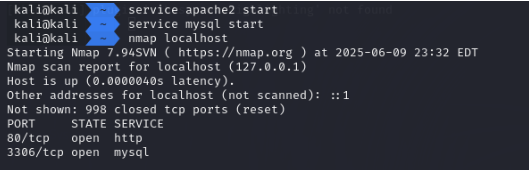
\includegraphics[width=0.7\textwidth]{./assets/img1.png}
	\caption{Verificación del estado de los servicios}
	\label{fig:servicios-estado}
\end{figure}

Ejecutamos el servicio de MySQL como usuario root:

\begin{figure}[H]
	\centering
	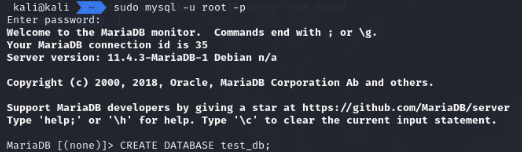
\includegraphics[width=0.7\textwidth]{./assets/img2.png}
	\caption{Acceso a MySQL como root}
	\label{fig:mysql-root}
\end{figure}

Creamos una base de datos para las pruebas:

\begin{figure}[H]
	\centering
	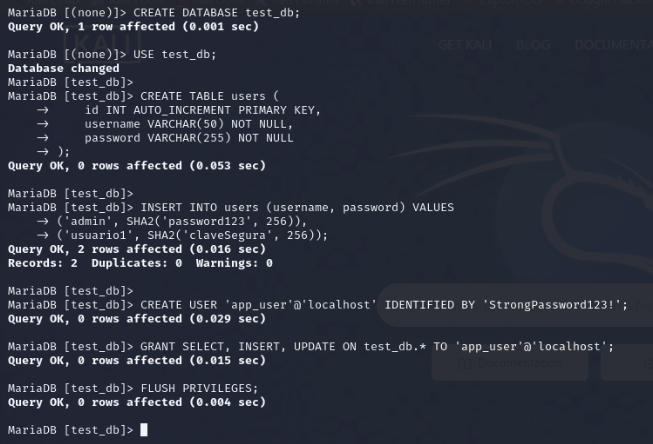
\includegraphics[width=0.7\textwidth]{./assets/img3.png}
	\caption{Creación de base de datos de prueba}
	\label{fig:db-creacion}
\end{figure}

\subsection{Implementación del Módulo de Seguridad}

**Archivo config.php - Módulo de Seguridad SQL**

\begin{figure}[H]
	\centering
	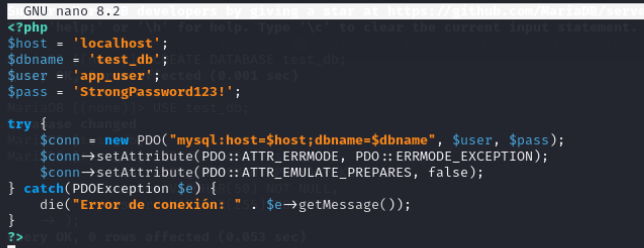
\includegraphics[width=0.75\textwidth]{./assets/img4.png}
	\caption{Implementación del módulo de seguridad contra SQL Injection}
	\label{fig:config-seguridad}
\end{figure}

Este archivo implementa las defensas contra SQL Injection e incluye:

\begin{itemize}
	\item Detección de patrones maliciosos (como UNION SELECT, DROP TABLE, comentarios
	      --)
	\item Escapado seguro de caracteres usando PDO::quote()
	\item Prepared statements con safeQuery(), que separa datos de código SQL
	\item Registro de intentos de ataque en logs para auditoría
\end{itemize}

\begin{figure}[H]
	\centering
	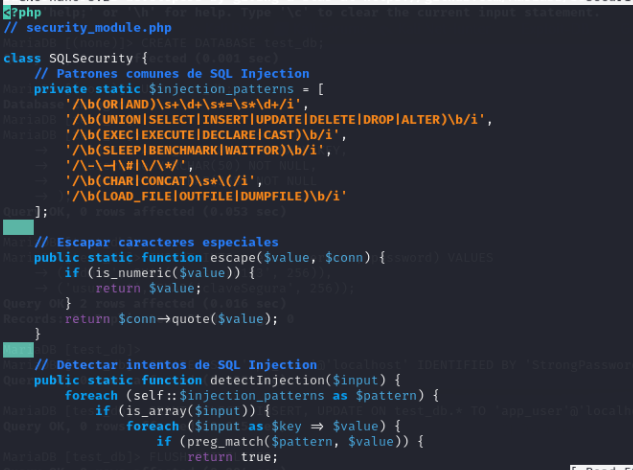
\includegraphics[width=0.75\textwidth]{./assets/img5.png}
	\caption{Código PHP - Funciones de seguridad (Parte 1)}
	\label{fig:php-seguridad-1}
\end{figure}

\begin{figure}[H]
	\centering
	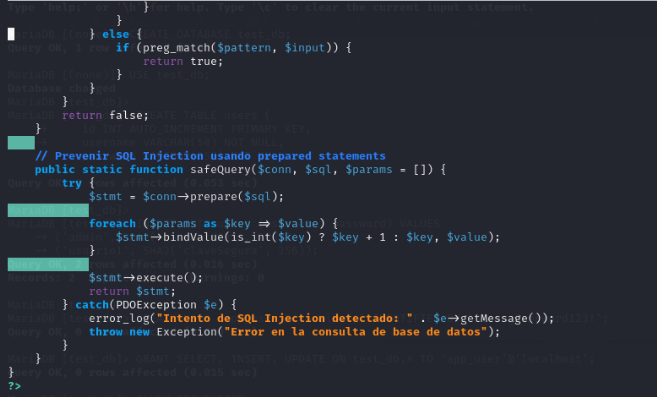
\includegraphics[width=0.75\textwidth]{./assets/img6.png}
	\caption{Código PHP - Funciones de seguridad (Parte 2)}
	\label{fig:php-seguridad-2}
\end{figure}

\subsection{Comparación: Código Vulnerable vs Código Seguro}

\**Login\_vulnerable.php** - Demuestra qué NO hacer: concatena inputs directamente en la consulta SQL sin sanitización, permitiendo que ataques como \texttt{admin' --} bypassen la autenticación. Muestra la consulta generada para evidenciar cómo la inyección modifica la lógica original (ej.: omite la verificación de contraseña). Es útil solo con fines educativos.

**Login\_seguro.php** - Aplica las contramedidas del módulo de seguridad:

\begin{figure}[H]
	\centering
	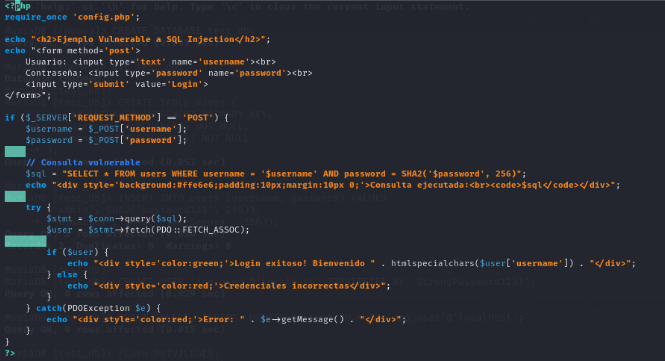
\includegraphics[width=0.75\textwidth]{./assets/img7.png}
	\caption{Login seguro - Implementación de contramedidas}
	\label{fig:login-seguro}
\end{figure}

Las características del login seguro incluyen:

\begin{itemize}
	\item Filtra inputs con \texttt{detectInjection()} (bloquea ataques conocidos)
	\item Usa prepared statements (\texttt{safeQuery()}) donde los parámetros se enlazan
	      de forma segura
	\item Nunca ejecuta inputs como código SQL, evitando que ataques como \texttt{' OR
		      1=1} tengan efecto
	\item Muestra la consulta "original" (con inputs) solo para comparación didáctica
\end{itemize}

\begin{figure}[H]
	\centering
	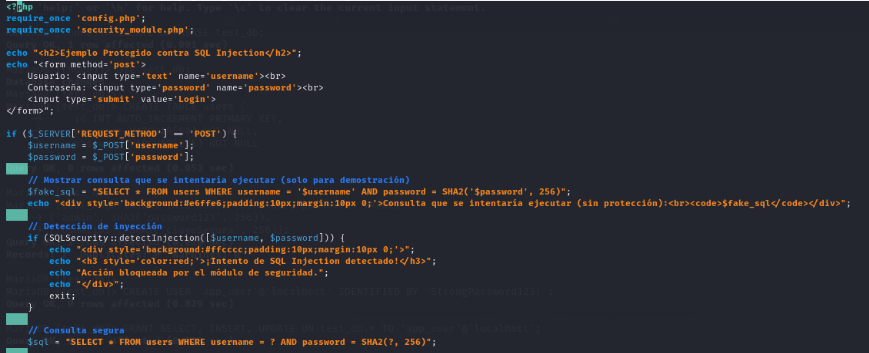
\includegraphics[width=0.75\textwidth]{./assets/img8.png}
	\caption{Código PHP - Implementación completa del login seguro}
	\label{fig:php-login-completo}
\end{figure}

\subsection{Pruebas de Vulnerabilidad}

Accedemos al servidor de Apache con \texttt{localhost/index.html}:

\begin{figure}[H]
	\centering
	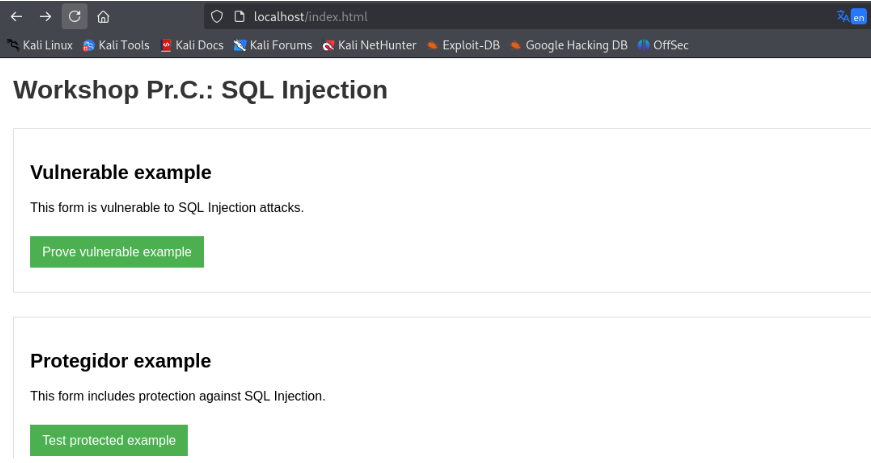
\includegraphics[width=0.7\textwidth]{./assets/img9.png}
	\caption{Interfaz web de pruebas}
	\label{fig:interfaz-web}
\end{figure}

\subsubsection{Pruebas en el Sistema Vulnerable}

Probamos el caso vulnerable con los siguientes datos:

\begin{lstlisting}[caption=Ataque SQL Injection - UNION SELECT]
Usuario: ' UNION SELECT 1, 'hacker', 'hash'-- 
Contraseña: [cualquier cosa]
\end{lstlisting}

\begin{figure}[H]
	\centering
	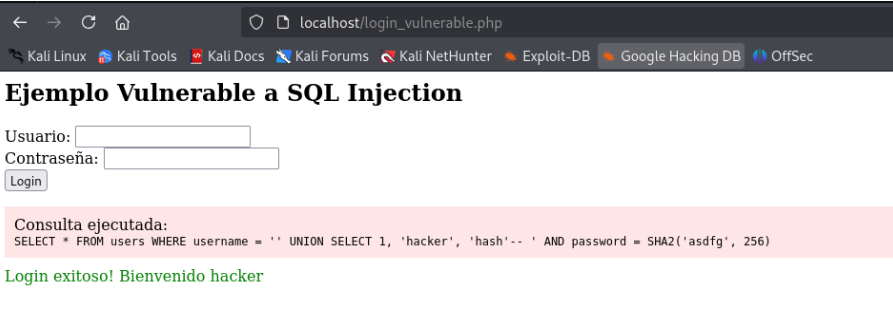
\includegraphics[width=0.7\textwidth]{./assets/img10.png}
	\caption{Resultado del ataque UNION SELECT en sistema vulnerable}
	\label{fig:ataque-union}
\end{figure}

Segunda prueba con bypass de autenticación:

\begin{lstlisting}[caption=Ataque SQL Injection - Bypass de autenticación]
Usuario: ' OR '1'='1
Contraseña: [cualquier cosa]
\end{lstlisting}

\begin{figure}[H]
	\centering
	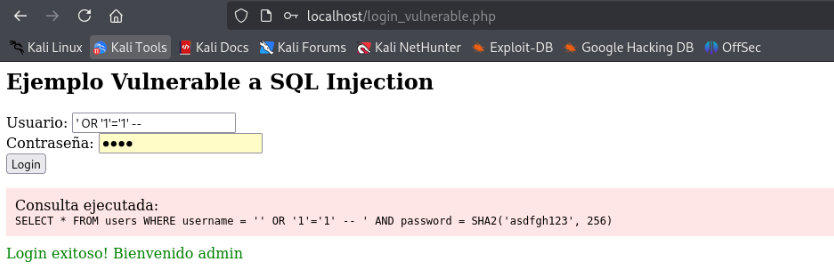
\includegraphics[width=0.7\textwidth]{./assets/img11.png}
	\caption{Resultado del bypass de autenticación en sistema vulnerable}
	\label{fig:bypass-vulnerable}
\end{figure}

\subsubsection{Pruebas en el Sistema Protegido}

Probamos los mismos ataques en el login protegido:

\begin{lstlisting}[caption=Intento de ataque UNION SELECT en sistema protegido]
Usuario: ' UNION SELECT 1, 'hacker', 'hash'-- 
Contraseña: [cualquier cosa]
\end{lstlisting}

\begin{figure}[H]
	\centering
	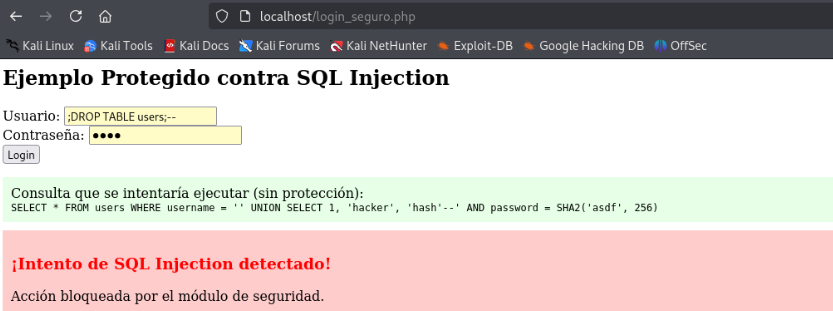
\includegraphics[width=0.7\textwidth]{./assets/img12.png}
	\caption{Bloqueo del ataque UNION SELECT en sistema protegido}
	\label{fig:proteccion-union}
\end{figure}

Segundo intento de ataque:

\begin{lstlisting}[caption=Intento de bypass en sistema protegido]
Usuario: ' OR '1'='1
Contraseña: [cualquier cosa]
\end{lstlisting}

\begin{figure}[H]
	\centering
	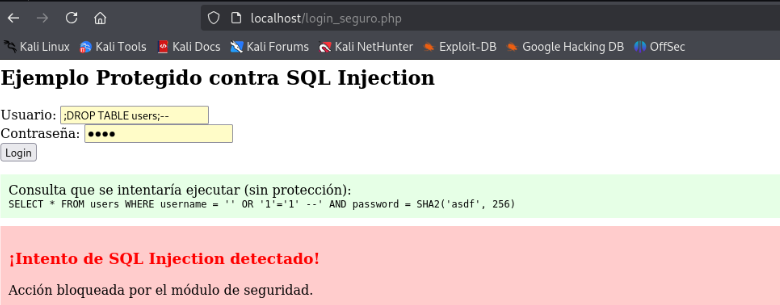
\includegraphics[width=0.7\textwidth]{./assets/img13.png}
	\caption{Bloqueo del bypass de autenticación en sistema protegido}
	\label{fig:proteccion-bypass}
\end{figure}

% ------------------------------------

\section{Conclusiones}

Este laboratorio ha presentado implementaciones prácticas de los principales
algoritmos criptográficos utilizados en la seguridad informática moderna. Las
implementaciones demuestran:

\begin{enumerate}
	\item La importancia de utilizar bibliotecas criptográficas probadas y seguras
	\item La necesidad de comprender las fortalezas y limitaciones de cada algoritmo
	\item La aplicación correcta de esquemas criptográficos para diferentes casos de uso
	\item La integración de múltiples técnicas para lograr seguridad completa
\end{enumerate}

\begin{securityalert}
	Estas implementaciones son con fines educativos. Para aplicaciones en producción, se recomienda realizar auditorías de seguridad adicionales y seguir los estándares de la industria como NIST y OWASP.
\end{securityalert}

\section{Referencias}

\begin{thebibliography}{9}

	\bibitem{nist2023}
	NIST,
	\textit{Recommendation for Key Management},
	Special Publication 800-57 Part 1 Rev. 5,
	2023.

	\bibitem{ferguson2010}
	N. Ferguson, B. Schneier, T. Kohno,
	\textit{Cryptography Engineering: Design Principles and Practical Applications},
	Wiley Publishing,
	2010.

	\bibitem{katz2014}
	J. Katz, Y. Lindell,
	\textit{Introduction to Modern Cryptography},
	Chapman and Hall/CRC,
	2nd Edition, 2014.

	\bibitem{menezes2018}
	A. Menezes, P. van Oorschot, S. Vanstone,
	\textit{Handbook of Applied Cryptography},
	CRC Press,
	2018.

	\bibitem{bernstein2009}
	D. Bernstein, T. Lange,
	\textit{Curve25519: New Diffie-Hellman Speed Records},
	Public Key Cryptography - PKC 2006,
	2009.

	\bibitem{cryptography2024}
	Python Cryptography Developers,
	\textit{Cryptography Documentation},
	\url{https://cryptography.io/en/latest/},
	2024.

\end{thebibliography}

\appendix

\section{Código Fuente Completo}

El código fuente completo de todas las implementaciones presentadas en este
laboratorio está disponible en el repositorio del curso. Para ejecutar los
ejemplos:

\begin{lstlisting}[language=bash, caption=Instalación y ejecución]
# Clonar repositorio
git clone https://github.com/universidad/lab-criptografia.git

# Instalar dependencias
pip install -r requirements.txt

# Ejecutar suite completa
python crypto_suite.py

# Ejecutar ejemplos individuales
python message_digest.py
python digital_signature.py
python symmetric_encryption.py
python asymmetric_encryption.py
python elliptic_curve.py
\end{lstlisting}

\section{Glosario}

\begin{description}
	\item[AES] Advanced Encryption Standard - Estándar de cifrado simétrico
	\item[CBC] Cipher Block Chaining - Modo de operación de cifrado por bloques
	\item[ECC] Elliptic Curve Cryptography - Criptografía de curvas elípticas
	\item[ECDH] Elliptic Curve Diffie-Hellman - Intercambio de claves con curvas
	      elípticas
	\item[ECDSA] Elliptic Curve Digital Signature Algorithm - Algoritmo de firma digital
	      con curvas elípticas
	\item[GCM] Galois/Counter Mode - Modo de cifrado autenticado
	\item[Hash] Función que mapea datos de tamaño arbitrario a tamaño fijo
	\item[HMAC] Hash-based Message Authentication Code - Código de autenticación basado
	      en hash
	\item[IV] Initialization Vector - Vector de inicialización
	\item[OAEP] Optimal Asymmetric Encryption Padding - Esquema de padding para RSA
	\item[PKCS] Public Key Cryptography Standards - Estándares de criptografía de clave
	      pública
	\item[RSA] Rivest-Shamir-Adleman - Algoritmo de cifrado asimétrico
	\item[SHA] Secure Hash Algorithm - Algoritmo de hash seguro
\end{description}

\end{document}